\documentclass[tikz]{standalone}
\usepackage{tikz}
\usepackage{fourier}
\usepackage{physics}
\usetikzlibrary{shapes.geometric}
\usetikzlibrary{calc}

\begin{document}
\begin{tikzpicture}
    % Spherical harmonic plots
    \node[inner sep=0] at (0, 0) {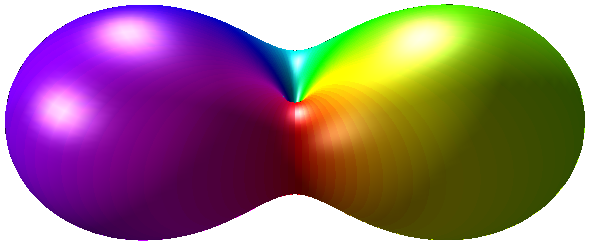
\includegraphics[scale=0.75]{../gfx/AFM-spherical.pdf}};
    \node[inner sep=0] at (7, 0) {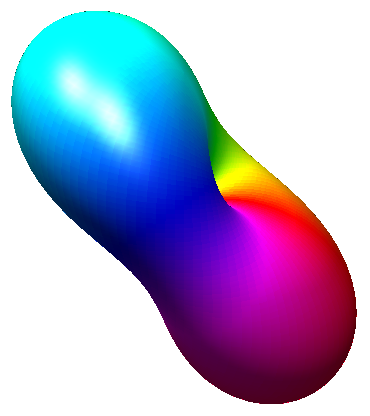
\includegraphics[scale=0.75]{../gfx/BA-spherical.pdf}};
         
    % Colour bar
    \node[rotate=90] at (-4.5, 0) {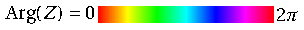
\includegraphics[scale=1.2]{../gfx/compiled_hsv.pdf}};

    % Labels
    \node at (-0.1, -3) {\large (a)};
    \node at (7, -3) {\large (b)};

    % Polar labels
    \draw[->, dashed, line width=1.5] (0, 0.3) -- (0, 2.2) node[above] {\large \(\langle\hat{\vb{F}}\rangle\)};
    \draw[->, dashed, line width=1.5] (7.35, 0.25) -- (8.55, 1.3) node[above] {\large \(\langle\hat{\vb{F}}\rangle\)};

    % Orientation
    \draw[->, line width=1.5] (-3.8, -3) -- (-3.8, -2) node[above] { \(z\)};
    \draw[->, line width=1.5] (-3.8, -3) -- (-2.8, -3) node[right] { \(x\)};
    \draw[->, line width=1.5] (-3.8, -3) -- (-3.2, -2.5) node[right] { \(y\)};

\end{tikzpicture}
\end{document}

